
\documentclass[12pt]{article} % Use A4 paper with a 12pt font size - different paper sizes will require manual recalculation of page margins and border positions

% Generated with LaTeXDraw 2.0.8
% Mon Jun 17 19:00:40 EDT 2013
\usepackage[usenames,dvipsnames]{pstricks}
\usepackage{epsfig}
\usepackage{pst-grad} % For gradients
\usepackage{pst-plot} % For axes
\usepackage[left=1.3cm,right=4.6cm,top=1.8cm,bottom=4.0cm,marginparwidth=3.4cm]{geometry} % Adjust page margins
\usepackage{amsmath} % Required for equation customization
\usepackage{amssymb} % Required to include mathematical symbols
\usepackage{xcolor} % Required to specify colors by name
\usepackage{amsthm}
\usepackage{float}
\usepackage{tikz}
\usetikzlibrary{shapes,backgrounds,trees}
\usepackage{wasysym}


\setlength{\parindent}{0cm} % Remove paragraph indentation
\newcommand{\tab}{\hspace*{2em}} % Defines a new command for some horizontal space
%\newcommand{\choose}[2]{\left(\begin{matrix}
%{#1}\\{#2}
%\end{matrix}\right)}

\title{Introduction to Probability Theory - Lecture 2}
%----------------------------------------------------------------------------------------

\newtheorem{defn}{Definition}
\newtheorem{example}{Example}
\newtheorem{prop}{Proposition}
\newtheorem{exer}{Exercises}
\newtheorem{thm}{Therorem}
\begin{document}
\maketitle
\section{Counting}
Now that we have a starting definition of probability in terms of the cardinality of sets, we need to learn to count outcomes (without explicitly enumerating them!)
\subsection{Tools for Counting}
Our primary tool for counting is something called the 'multiplication rule'. Before we state it, lets look at a couple of examples.
\begin{example}
Consider an experiment where we roll two dice - one white, one blue (I want them to be \emph{distinguishable} - more on that later). How many possible outcomes are there? \\\\
% Set the overall layout of the tree
%\tikzstyle{level 1}=[level distance=3.5cm, sibling distance=3.5cm]
%\tikzstyle{level 2}=[level distance=3.5cm, sibling distance=2cm]

% Define styles for bags and leafs
\tikzstyle{Blue} = [text width=4em, text centered]
\tikzstyle{Trt} = [text width=4em, text centered]
%\tikzstyle{end} = [circle,fill]

% The sloped option gives rotated edge labels. Personally
% I find sloped labels a bit difficult to read. Remove the sloped options
% to get horizontal labels. 


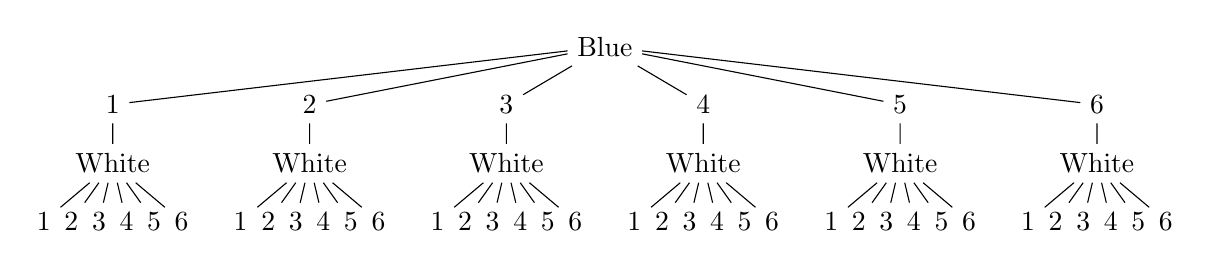
\begin{tikzpicture}[grow=down, sloped,every node/.style = {},level distance=.5cm,
level 1/.style={sibling distance=2.5cm},
level 2/.style={sibling distance=.35cm}]
\node[](Blue){Blue}
  child foreach \y in {1,2,3,4,5,6} {
        node[below](\y a) {\y}
        child {
              node[below](White){White}
                  child foreach \x in {1,2,3,4,5,6} {
                        node[below](\x){\x}
                        edge from parent
              }           
              edge from parent
        } 
        edge from parent                
};
   
\end{tikzpicture}
\end{example}

%\begin{example}
%Suppose we have $2$ treatments and $3$ patients (not realistic, but we want the number small so we can draw a picture). We will randomly assign each patient to a treatment group, and each patient in each group will either get drug or placebo. How many possible outcomes are there? \\\\
%\begin{tikzpicture}[grow=down, sloped,every node/.style = {},level distance=.8cm,
%level 1/.style={sibling distance=5.5cm},
%level 2/.style={sibling distance=9.35cm},level 3/.style={sibling %distance=1.5cm},level 4/.style={sibling distance=.9cm}]
%\node[](Trt){Treatment}
 % child foreach \y in {1,2} {
 %       node[below](\y a) {\y}
 %       child {
 %             node[below](Pt){Patient}
 %                 child foreach \x in {1,2,3} {
 %                       node[below](\x){\x}
 %                           child foreach \z in {0,1} {
 %                               node[below] (\z b){\z}
                               % edge from parent
  %                          }
  %                 %     edge from parent
  %            }           
  %          %  edge from parent
 %       } 
     %   edge from parent                
%};
   
%\end{tikzpicture}

%\end{example}
Now we are ready to state the multiplication rule: In a compound experiment, if one experiment has $m$ outcomes and the other has $n$ outcomes, the total number of outcomes is $m\cdot n$. In general, if we have a compound experiment made up of $k$ experiments, there are 
$$n_1\cdot n_2\cdot...\cdot n_k$$
possible outcomes. Similarly, if an experiment has $n$ possible outcomes and we perform $r$ trials, there are $n^r$ possible outcomes in total.
\subsection{Sampling with and without Replacement}
Many probability problems can be cast as 'sampling'. I.e., we have an urn of colored balls and select some of them by some procedure. So, suppose we have such and urn, say with $k$ balls, and for now, all of \emph{different} colors. We decide to take out $k\leq n$ colored balls and record the result. There are a few ways to do this.\\

Suppose we take out one ball, record its color and the \emph{replace} it to the urn. Then we take a second ball, record the color, replace, etc. This is called, rather appropriately, sampling \emph{with replacement}.\\

On the other hand, we could take out a ball, record its color, and then put it aside and select the next ball. This is called sampling \emph{without replacement}. \\

The number of outcomes of these two experiments is different. 
\subsubsection{With Replacement}
Sampling with replacement is the same as performing $k$ trials of an experiment that has $n$ possible outcomes. If we have an urn containing $n$ \emph{distinguishable} objects (say each one has a unique label), and we select $k$ objects one at a time, with replacement, the number of possible outcomes is given by:
$$n^k$$
This is obtained by applying the multiplication rule: there are $n$ outcomes for the first selection, and still $n$ outcomes for each succeeding selection.

\subsubsection{Without Replacement}
When we sample without replacement, the number of possible outcomes decreases with each selection. If we have $n$ objects and we select $k$ of them, one at a time, the first choice has $n$ possibilities, the second has $n-1$ possibilities, the third $n-2$ and so on, up to $n-k+1$. By the multiplication rule, then, the number of possible outcomes is:
$$n(n-1)(n-2)...(n-k+1)$$
\begin{example}
A lottery drawing consists choosing $5$ of $45$ numbered balls (numbered $1-45$) and a winning ticket predicts the five digits \emph{in the order they are selected}. How many possible outcomes are there?
$$45\cdot44\cdot43\cdot42\cdot41 = \textrm{ a lot!}$$ 
\end{example}
\subsubsection{Permutations}
A special case of sampling without replacement is something called a permutation. A permutation is a reordering of a collection of objects. For example consider the set
$$\left\{1,2,3,4,5\right\}$$
A permutation of this set would be:
$$\left\{2,5,4,1,3\right\}$$
Another permutation might be:
$$\left\{1,2,3,5,4\right\}$$
This can be seen as sampling without replacement, because we can see the reordering as choosing one of the five numbers as the first number, then one of the four remaining as the second, and so on. Once we choose a number, it is 'removed' from the set of objects. Thus, the number of permutations of the set 
$$\left\{1,2,3,4,5\right\}$$
is given by 
$$5\cdot4\cdot3\cdot2\cdot1 = 5!$$
In general, the number of ways to permute $n$ \emph{distinguishable} objects is $n!$.\\
This brings us to an important concept in counting outcomes.
\subsection{Distinguishable and Indistinguishable Objects/Outcomes}
We have seen that when the $n$ objects in a collection are \emph{distinguishable}, the number of possible orderings is $n!$. (By \emph{distinguishable}, we mean the objects are uniquely identifiable.) Suppose some of the objects in a collection are \emph{indistinguishable}? Consider:
$$a,b,b$$
How many orderings of this collection? First, let's label one of the $b's$. Consider
$$a,b,b^*$$
Now, we have 3 distinguishable objects and so there are $3!=6$ orderings:\\\\

$$\begin{matrix}a,b,b^* &b,a,b^*& b,b^*,a\\
              a,b^*,b&b^*,a,b&b^*,b,a
\end{matrix}$$
If we remove the labels, we see that we have over-counted by the number of permutations of the indistinguishable objects. Thus, the number of orderings is:
$$\frac{3!}{2!}$$
In general, the number of ways to arrange $n$ objects, when $k$ of those are indistinguishable is:
$$\frac{n!}{k!}$$
Even more generally, the number of ways to arrange $n$ objects, $k_1$ of which are of one type, $k_2$ another, and so on up to $k_r$ is given by:
$$\frac{n!}{k_1!k_2!...k_r!}$$
\subsection{Combinations}
Now, instead of rearranging, lets return to choosing $k$ objects from $n$ objects without replacement. Assuming distinguishable objects, the number of possible outcomes is:
$$n(n-1)...(n-k+1)$$
Suppose we do not care about the order of the choices. How many outcomes? We take the number of outcomes with orderings, and divide by the number of permutations of the $k$ objects. I.e.
$$\frac{n(n-1)...(n-k+1)}{k!}$$
Rearranging, we can write this as:
$$\frac{n!}{(n-k)!k!} \equiv {n\choose{k}}$$
we read
$$n\choose{k}$$ 
as '$n$ choose $k$'. Note that the book calls combinations 'binomial coefficients'. This is because of their occurrence in the binomial expansion:
$$\left(x+y\right)^n = \sum_{k=0}^n {n\choose{k}} x^ky^{n-k}$$

\end{document}